% Notes on the dissipative ferromagnetic scar tower: what has been found so far.
% Build:  cd latex && latexmk -pdf notes.tex
% Figures are copies of the outputs in data/ (not tracked by git); regenerate them with the
% scripts named in each caption and copy them to latex/figures/.

\documentclass[11pt,a4paper]{article}
\usepackage[margin=2.3cm]{geometry}
\usepackage{amsmath,amssymb}
\usepackage{graphicx}
\usepackage{booktabs}
\usepackage{xcolor}
\usepackage{dsfont}
\usepackage[colorlinks=true,linkcolor=blue!50!black,citecolor=blue!50!black,urlcolor=blue!50!black]{hyperref}

\graphicspath{{figures/}}

\newcommand{\ket}[1]{\lvert #1 \rangle}
\newcommand{\bra}[1]{\langle #1 \rvert}
\newcommand{\dyad}[2]{\lvert #1 \rangle\!\langle #2 \rvert}
\newcommand{\Tr}{\operatorname{Tr}}
\newcommand{\Ptow}{P_{\mathrm{tower}}}
\newcommand{\Lv}{\mathcal{L}}
\newcommand{\D}{\mathcal{D}}

\title{Ferromagnetic scar tower under bulk dephasing:\\ notes on the results so far}
\author{Weyner Ccuiro}
\date{14 October 2026}

\begin{document}
\maketitle

\begin{abstract}
We study how the ferromagnetic quantum many-body scar tower of a spin-$1/2$ chain decays under uniform $\sigma^z$ dephasing, using exact density-matrix evolution and full Liouvillian diagonalization for $L \le 8$. The coherent oscillations launched from the scar state $\ket{-}^{\otimes L}$ decay at a rate that grows roughly linearly with $L$ ($\Gamma \approx 0.8\,\gamma L$ in a fixed fit window), whereas non-scar probes (energy autocorrelation and a staggered transverse magnetization) decay at rates close to the single-spin value $2\gamma$ with weak or no $L$-dependence. At fixed $L = 6$ all rates are linear in $\gamma$ for weak dephasing; for strong dephasing the scar rate falls back to $2\gamma$. Several exact results organize the data: the two fully polarized states are dark states, so the steady state is three-fold degenerate, and the edge coherences of the tower are exact Liouvillian eigenmodes with $\operatorname{Re}\lambda = -2n\gamma$ for every $L$.
\end{abstract}

\tableofcontents

%======================================================================
\section{Model}

\paragraph{Hamiltonian.} Spin-$1/2$ ring of $L$ sites (periodic boundaries), $S^\alpha_j = \sigma^\alpha_j/2$, bond singlet projector $R_{j,j+1} = \tfrac14 - \mathbf S_j\cdot\mathbf S_{j+1}$:
\begin{equation}
H = H_I + h S^z_{\mathrm{tot}}, \qquad
H_I = \sum_j \Big[ \sum_\alpha \big( a_\alpha R_{j,j+1}\sigma^\alpha_{j+2} + b_\alpha \sigma^\alpha_{j-1}R_{j,j+1} \big)
+ \sum_{\alpha\beta} c^{(j)}_{\alpha\beta}\, \sigma^\beta_{j-1} R_{j,j+1} \sigma^\alpha_{j+2} \Big].
\end{equation}
Every term of $H_I$ annihilates the ferromagnetic multiplet $\ket{\Phi_n} \propto (S^-_{\mathrm{tot}})^n\ket{\uparrow\cdots\uparrow}$, $n = 0,\dots,L$, so $H\ket{\Phi_n} = h(L/2-n)\ket{\Phi_n}$: an equally spaced tower of $L+1$ exact scars. Coefficients: $h = 0.5$, $a = (0.73, 0.41, 0.29)$, $b = (0.58, -0.37, 0.66)$; the only nonzero $c$ are $c_{xz}, c_{zy}, c_{yx}$ with baseline values $0.31, -0.44, 0.27$.

\paragraph{Random $c$.} To remove translation symmetry, each nonzero $c_{\alpha\beta}$ is multiplied on every bond $j$ by an independent factor uniform in $[0.5, 1.5]$ (signs and scale kept; $a$, $b$ uniform). One realization per $L$ (seed $1000\cdot 1 + L$), shared by all runs below unless stated otherwise. Every term still annihilates the tower.

\paragraph{Dephasing.}
\begin{equation}
\dot\rho = \Lv\rho = -i[H,\rho] + \gamma\sum_j \big(\sigma^z_j\rho\,\sigma^z_j - \rho\big).
\end{equation}
In the Pauli basis $\rho = 2^{-L}\sum_P r_P P$ the dissipator is diagonal, $\D(P) = -2\gamma\, n_{xy}(P)\, P$, with $n_{xy}(P)$ the number of sites carrying $\sigma^x$ or $\sigma^y$. A single spin's transverse coherence decays as $e^{-2\gamma t}$.

\paragraph{Initial states.} The scar state $\ket{-}^{\otimes L}$ (all spins along $-x$), which lies entirely in the tower, and product states on a cone around $-x$: spin $j$ along $(-\cos\theta, \sin\theta\cos\varphi_j, \sin\theta\sin\varphi_j)$ with random $\varphi_j$; $\theta = 0$ is the scar state.

\paragraph{Methods.} (i) Exact evolution of the real Pauli-coefficient vector, $\exp(\Lv\,dt)$ by a Taylor series summed to round-off; translation orbits for the uniform model ($\dim\approx 4^L/L$), the full Pauli basis ($4^L$) for random $c$. (ii) Full exact diagonalization of the dense $4^L\times4^L$ real generator (LAPACK \texttt{dgeev}, Intel MKL) for $L\le 6$; at $\gamma = 0$ the Liouvillian is degenerate, so $H$ is diagonalized instead and the modes are $\dyad{m}{n}$, $\lambda = -i(E_m-E_n)$.

%======================================================================
\section{Exact results}

\paragraph{Dark states and steady states.} $\ket{\Phi_0} = \ket{\uparrow\cdots\uparrow}$ and $\ket{\Phi_L} = \ket{\downarrow\cdots\downarrow}$ are eigenstates of $H$ and of every $\sigma^z_j$, hence dark states of the dissipator. The kernel of $\Lv$ is spanned by
\begin{equation}
\mathds{1}, \qquad \dyad{\Phi_0}{\Phi_0}, \qquad \dyad{\Phi_L}{\Phi_L},
\end{equation}
and ED finds exactly three zero eigenvalues for $L = 4, 5, 6$. The infinite-temperature state is therefore \emph{not} the unique steady state. The coherence $\dyad{\Phi_0}{\Phi_L}$ is an eigenmode with $\lambda = -2\gamma L - ihL$, which saturates the general bound $-2\gamma L \le \operatorname{Re}\lambda \le 0$.

\paragraph{Edge coherences of the tower.} Since $\sigma^z_j\ket{\Phi_0} = \ket{\Phi_0}$ and $\sum_j\sigma^z_j = 2S^z_{\mathrm{tot}}$,
\begin{equation}
\D\big(\dyad{\Phi_0}{\Phi_n}\big) = \gamma\,\dyad{\Phi_0}{\Phi_n}\Big(\sum_j\sigma^z_j - L\Big) = -2n\gamma\,\dyad{\Phi_0}{\Phi_n},
\end{equation}
and both states are eigenstates of $H$, so $\dyad{\Phi_0}{\Phi_n}$ (and likewise $\dyad{\Phi_L}{\Phi_{L-n}}$) is an exact Liouvillian eigenmode with
\begin{equation}
\lambda = -2n\gamma - i h n \qquad \text{for every } L.
\end{equation}
The slowest tower modes therefore decay at exactly $2\gamma$, independent of $L$; ED confirms four modes at $-\operatorname{Re}\lambda = 2\gamma$ for each $L$. In first-order perturbation theory the coherences $\dyad{\Phi_n}{\Phi_{n+1}}$ decay at $\gamma L(1 - m_n m_{n+1})$ with $m_n = 1 - 2n/L$: $2\gamma$ at the edges, $\approx\gamma L$ in the middle of the tower. The scar signal is a binomially weighted sum of these, which makes it multi-exponential (Sec.~\ref{sec:scaling}).

\paragraph{Initial loss of tower weight.} For $\rho = \dyad{\psi}{\psi}$ with $\ket\psi = \ket{-}^{\otimes L}$, $w = \Tr(\Ptow\rho)$ and $[\Ptow,H] = 0$,
\begin{equation}
\dot w(0) = \gamma\sum_j\big(\lVert\Ptow\sigma^z_j\ket\psi\rVert^2 - 1\big), \qquad
\Ptow\sigma^z_j\ket\psi = \tfrac{2}{L}S^z_{\mathrm{tot}}\ket\psi
\;\Rightarrow\; \dot w(0) = -\gamma(L-1),
\end{equation}
using permutation symmetry of the tower and $\langle (S^z_{\mathrm{tot}})^2\rangle = L/4$. Reproduced exactly by the numerics for $L = 4,\dots,8$. At late times $w \to (L+1)/2^L$.

\paragraph{Overlaps of the probes.} $\Ptow\sigma^x_j\Ptow = \tfrac2L S^x_{\mathrm{tot}}\Ptow$ for every $j$, so $O_k = \sum_j e^{ikj}\sigma^x_j$ has zero tower part for $k \neq 0$. The single-site $\sigma^x$ content of $H$ is $\tfrac14(a_x+b_x)\sum_j\sigma^x_j$ (the $c$ terms contain none), so $\Tr(O_k H) = 0$ exactly for $k\neq0$ even with random $c$. Since $\Ptow H\Ptow = hS^z_{\mathrm{tot}}\Ptow$ and $[\Ptow,H]=0$, the operator $\tilde H = H - hS^z_{\mathrm{tot}}\Ptow = (1-\Ptow)H(1-\Ptow)$ is conserved at $\gamma=0$ and has no tower component.

\paragraph{$S^z$ is not conserved, but does not relax to the tower value.} At $\gamma=0$, $\langle\sigma^z\rangle$ from a cone state relaxes only partially (for $L=5$, $\theta=\pi/2$: from $0.279$ to a late-time mean $\approx0.15$), while its tower part is only $\tfrac2L\Tr(\Ptow S^z_{\mathrm{tot}}\rho_0) = 0.031$. The difference is the thermal value of the bulk: $H$ contains $hS^z_{\mathrm{tot}}$, so energy conservation fixes a nonzero $S^z$.

%======================================================================
\section{Scar oscillations and their decay}

\paragraph{Noiseless check.} At $\gamma = 0$ the scar state precesses perfectly, $\langle\sigma^x_j\rangle = -\cos ht$, $\langle\sigma^y_j\rangle = -\sin ht$, on every site and for every $L$ (deviation $\lesssim 10^{-13}$), with uniform or random $c$.

\paragraph{Decay against $L$.} The amplitude $m_\perp = \sqrt{m_x^2+m_y^2}$ decays faster for larger $L$ (Fig.~\ref{fig:baseline}). For the translation-invariant model, fitting $e^{-\Gamma t}$ while $m_\perp > 0.05$ gives the rates in Table~\ref{tab:baseline}, well described by $\Gamma \approx 0.63\,\gamma L^{1.13}$. Breaking translation with random $c$ changes them by less than $2\%$.

\begin{table}[h]
\centering
\begin{tabular}{lccccccc}
\toprule
$L$ & 4 & 5 & 6 & 7 & 8 & 9 & 10 \\
\midrule
$\Gamma/\gamma$, uniform $c$ & 3.06 & 3.80 & 4.66 & 5.75 & 6.68 & 7.61 & 8.39 \\
$\Gamma/\gamma$, random $c$  & 3.06 & 3.89 & 4.68 & 5.81 & 6.69 & -- & -- \\
\bottomrule
\end{tabular}
\caption{Scar decay rate at $\gamma = 0.01$, fit window $m_\perp > 0.05$.}
\label{tab:baseline}
\end{table}

\begin{figure}[h]
\centering
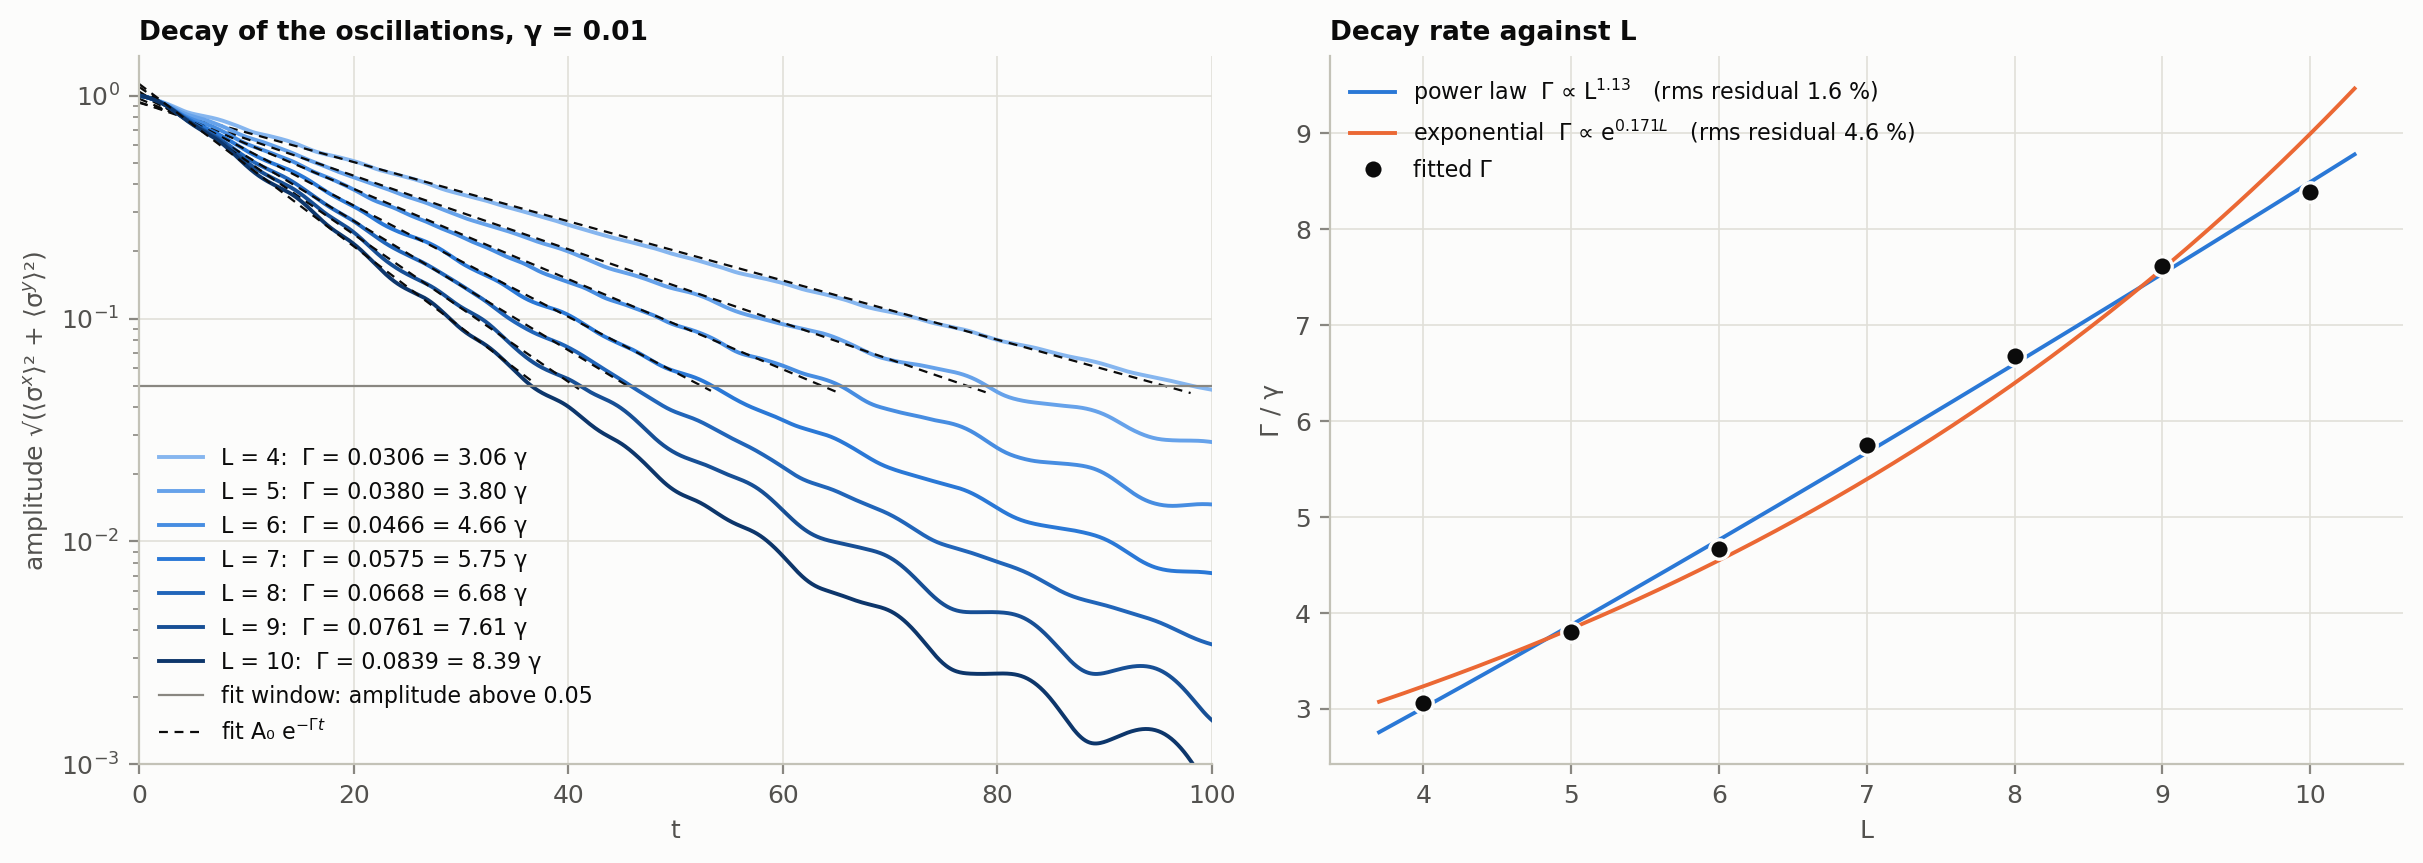
\includegraphics[width=\textwidth]{decay_fit.png}
\caption{Uniform model, $\gamma = 0.01$: decay of $m_\perp$ from $\ket{-}^{\otimes L}$ for $L = 4,\dots,10$ and the fitted rate against $L$ (\texttt{plot\_scripts/fit\_decay.py}).}
\label{fig:baseline}
\end{figure}

\paragraph{Cone states.} Starting off the tower (Fig.~\ref{fig:cone}), the oscillations of $\langle\sigma^x\rangle$ survive at $\gamma = 0$ with reduced amplitude for small tilt ($\theta = \pi/8, \pi/4$) and are essentially gone for $\theta \ge 3\pi/8$, $L\ge5$; with dephasing they die within a few periods. At small $L$ the site averages carry a sampling offset from the random azimuths, $\sin\theta\,\overline{\cos\varphi_j}$ and $\sin\theta\,\overline{\sin\varphi_j}$.

\begin{figure}[h]
\centering
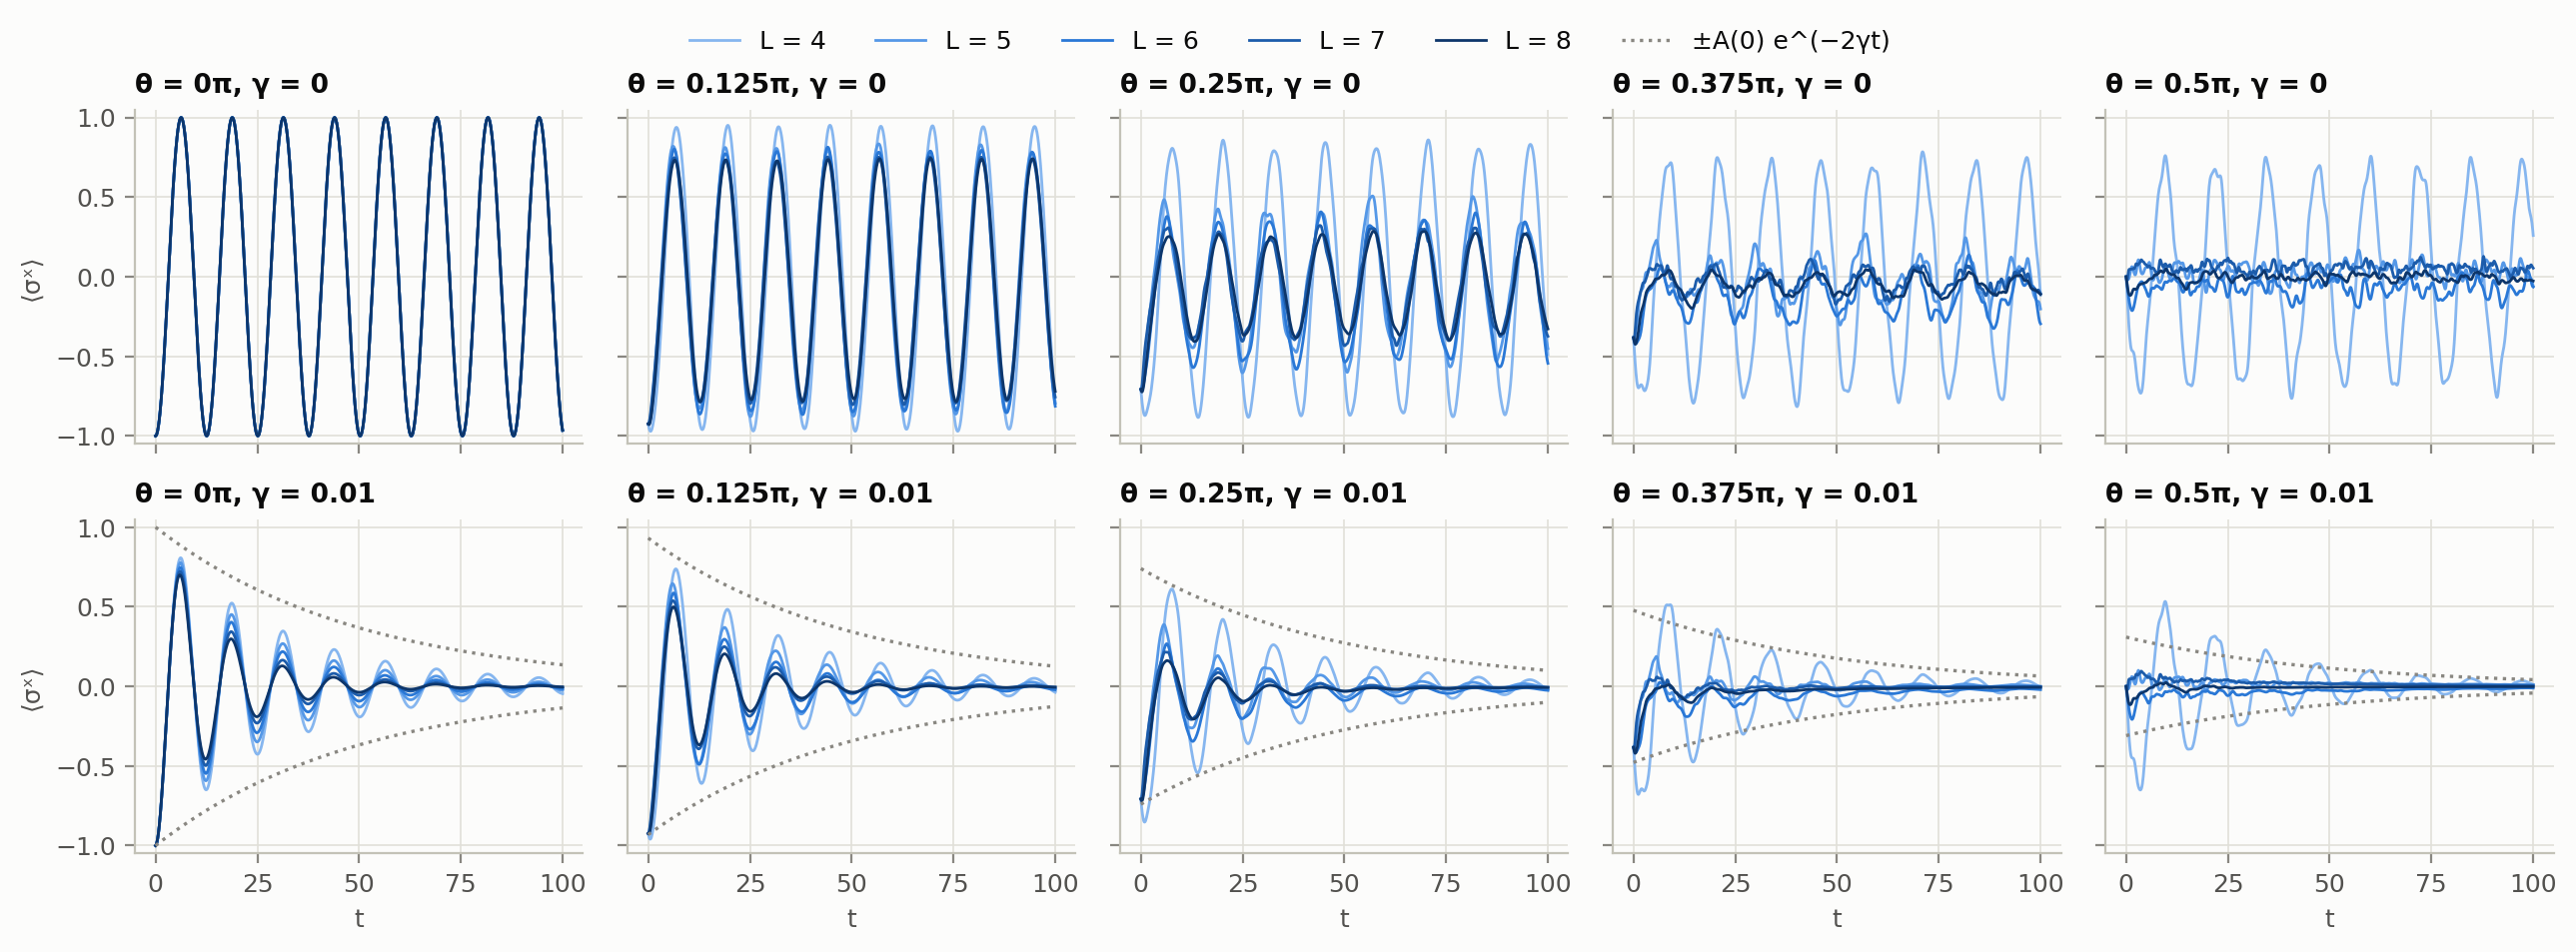
\includegraphics[width=\textwidth]{disorder_mx.png}
\caption{Random $c$: site-averaged $\langle\sigma^x\rangle$ from cone states with random azimuths, $\gamma = 0$ (top) and $0.01$ (bottom); dotted: free-spin envelope (\texttt{plot\_scripts/plot\_disorder.py}).}
\label{fig:cone}
\end{figure}

%======================================================================
\section{Scar versus non-scar probes}
\label{sec:scaling}

Three probes, evolved with the same Lindbladian (random $c$, $L = 4,\dots,8$, $\gamma = 0$ and $0.01$):
\begin{itemize}
\item \textbf{P1, scar:} $m_\perp(t)$ from $\rho_0 = \dyad{-}{-}^{\otimes L}$.
\item \textbf{P2, energy:} $C(t) = \Tr[\tilde H e^{\Lv^\dagger t}(\tilde H)]/\Tr\tilde H^2$, conserved at $\gamma = 0$.
\item \textbf{P3, thermal:} $|C^+(t)|$ for $O^+ = \sum_j(-1)^j\sigma^+_j$ ($k=\pi$, even $L$), built from separate evolutions of $O^x_\pi$ and $O^y_\pi$ so that the precession in $h$ drops out. At $\gamma=0$ it thermalizes by $t\approx1$ and then sits at a finite-size floor ($0.17, 0.05, 0.015$ for $L = 4, 6, 8$). Its dephasing rate is $\Delta\Gamma$, the slope of $-\ln(|C^+_\gamma|/|C^+_0|)$ on a common short window.
\end{itemize}

\begin{figure}[h]
\centering
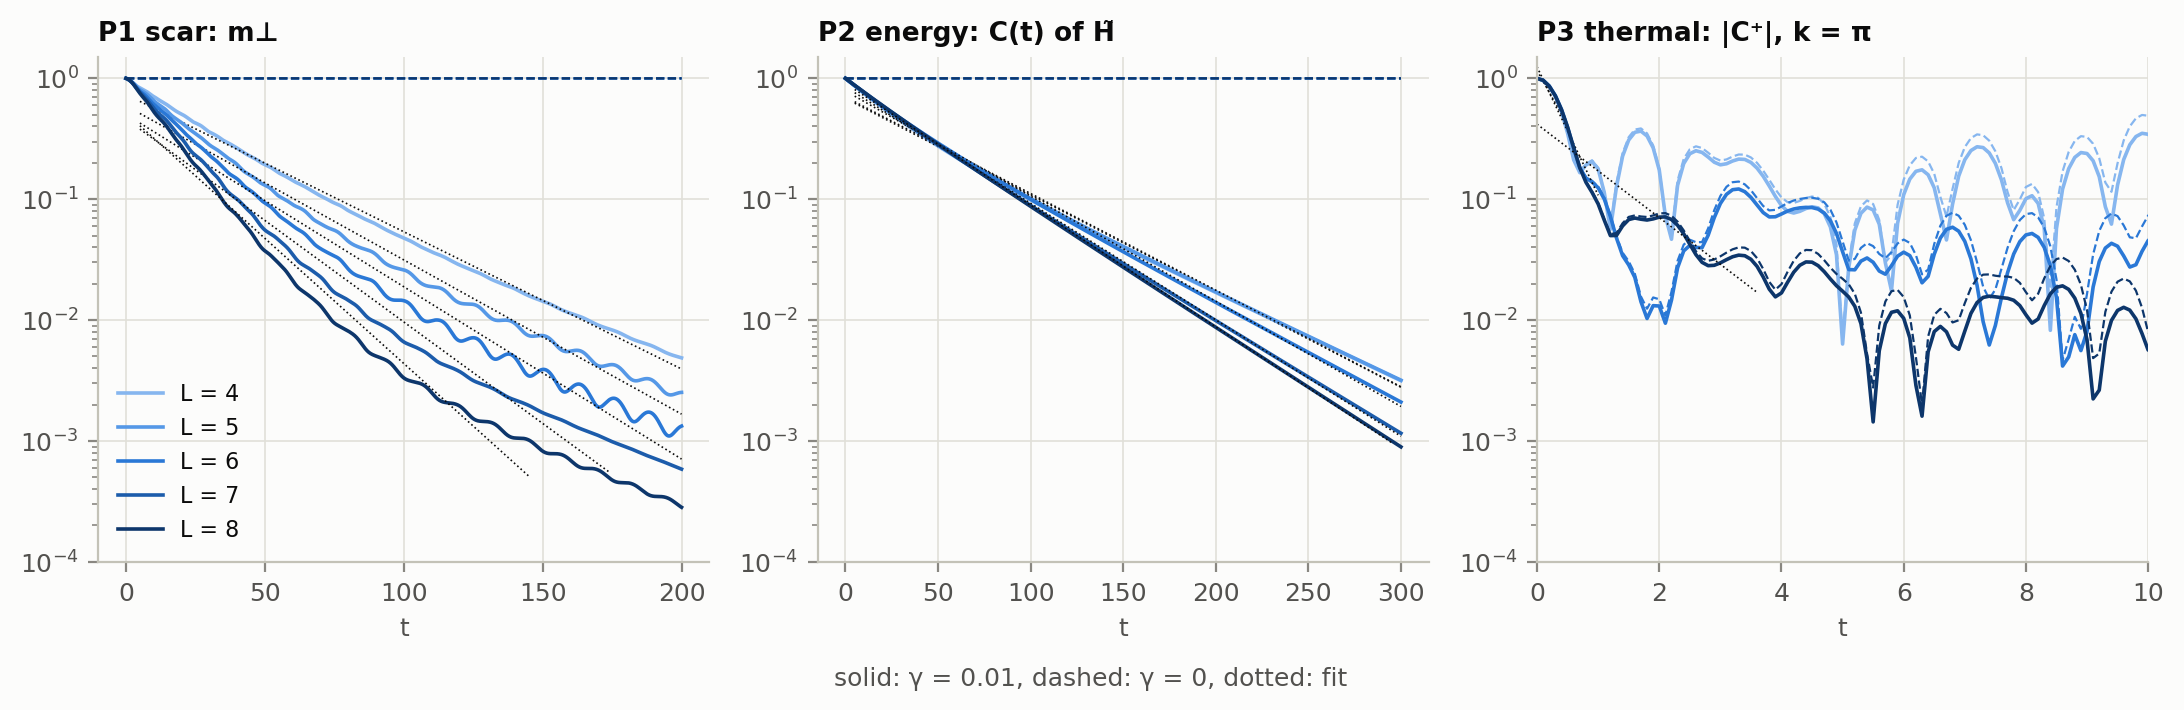
\includegraphics[width=\textwidth]{probe_timeseries.png}
\caption{The three probes against time, $\gamma = 0.01$ (solid) and $\gamma = 0$ (dashed); dotted lines are the fits (\texttt{plot\_scripts/fit\_probes.py}).}
\label{fig:probes}
\end{figure}

\paragraph{Scaling with $L$.} Table~\ref{tab:scaling} and Fig.~\ref{fig:scaling}. The scar rate grows close to linearly in $L$; the non-scar rates stay near the single-spin value $2\gamma$ with a weak (energy) or no (thermal) $L$-dependence.

\begin{table}[h]
\centering
\begin{tabular}{lcccccc}
\toprule
probe ($\Gamma/\gamma$) & $L=4$ & 5 & 6 & 7 & 8 & power law \\
\midrule
P1 scar, window $t\in[5,60]$            & 3.22 & 4.01 & 4.69 & 5.67 & 6.51 & $L^{1.01\pm0.03}$ \\
P1 scar, window $t\in[5, m_\perp=10^{-3}]$ & 2.61 & 2.94 & 3.28 & 3.87 & 4.77 & $L^{0.84\pm0.12}$ \\
P2 energy $\tilde H$                    & 1.83 & 1.84 & 2.00 & 2.22 & 2.32 & $L^{0.37\pm0.07}$ \\
P3 thermal $\Delta\Gamma$, $t\in[0,0.5]$ & 1.43 & -- & 1.59 & -- & 1.61 & $L^{0.18\pm0.06}$ \\
P3 thermal $\Delta\Gamma$, $t\in[0,1]$   & 2.25 & -- & 2.25 & -- & 1.85 & $L^{-0.27\pm0.19}$ \\
\bottomrule
\end{tabular}
\caption{Decay rates at $\gamma = 0.01$ (random $c$) and power-law fits $\Gamma = aL^b$.}
\label{tab:scaling}
\end{table}

\begin{figure}[h]
\centering
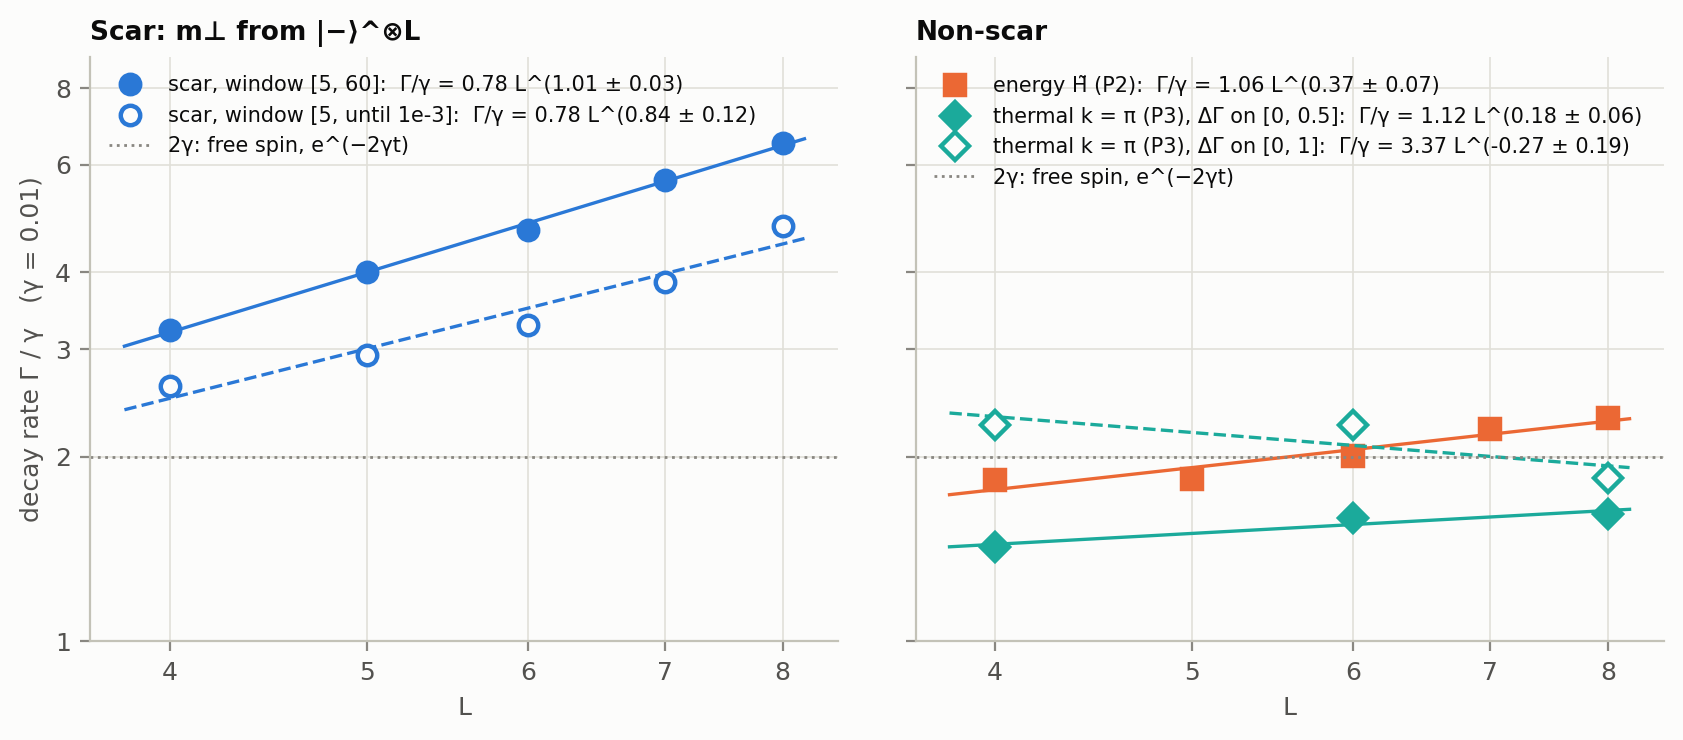
\includegraphics[width=\textwidth]{probe_scaling.png}
\caption{Decay rate against $L$ (log-log) with power-law fits; scar (left) and non-scar probes (right).}
\label{fig:scaling}
\end{figure}

\paragraph{Caveats.}
\begin{itemize}
\item The scar decay is multi-exponential (Fig.~\ref{fig:probes}, left): mid-tower coherences ($\sim\gamma L$) dominate early, the exact $2\gamma$ edge modes late. $\Gamma_{\mathrm{scar}}$ and its $L$-exponent depend on the fit window.
\item $L = 4,\dots,8$ is a factor of two in $L$: power law and exponential fit about equally well; the exponents are descriptive.
\item One disorder realization per $L$.
\item For P3, a window that ends at twice the noise floor lengthens with $L$ and produces a spurious growth of $\Delta\Gamma$ ($1.43, 2.25, 4.39$); only common windows are meaningful.
\item The predicted initial rate of P2, $2\gamma\sum_P n_{xy}h_P^2/\sum_P h_P^2$, is $2.7$--$2.9\,\gamma$; the long-time decay is slower ($1.8$--$2.3\,\gamma$).
\end{itemize}

%======================================================================
\section{Liouvillian spectrum}

Full ED at $\gamma = 0.01$ for $L = 4, 5, 6$ (Fig.~\ref{fig:spectrum}). Each right eigenvector $R$ is split into tower ($\lVert\Ptow R\Ptow\rVert$), mixed and bulk weights. Findings:
\begin{itemize}
\item three zero modes (Sec.~2), and $\operatorname{Re}\lambda \ge -2\gamma L$ saturated by $\dyad{\Phi_0}{\Phi_L}$;
\item the bulk is centred at $-\operatorname{Re}\lambda\approx\gamma L$ (the mean dephasing rate of a Pauli string);
\item the slowest tower modes sit at exactly $2\gamma$ (edge coherences); the next ones at $4\gamma$ for $L = 5, 6$ ($2.94\gamma$ at $L = 4$);
\item the slowest bulk mode is at $1.67\gamma$, $1.66\gamma$, $1.88\gamma$ for $L = 4,5,6$, comparable to the P2 rate;
\item modes with tower weight $>0.9$: 22 of 25, 32 of 36, 38 of 49: at $\gamma=0.01$ some tower coherences already hybridize with the bulk.
\end{itemize}
Checks: at $\gamma = 0$ the dense spectrum equals $-i(E_m - E_n)$ to $5\times10^{-14}$ ($L = 4, 5$); $\sum\lambda = \Tr\Lv = -\gamma L4^L$; $L+1$ eigenstates of $H$ in the tower at energies $h(L/2-n)$.

\begin{figure}[h]
\centering
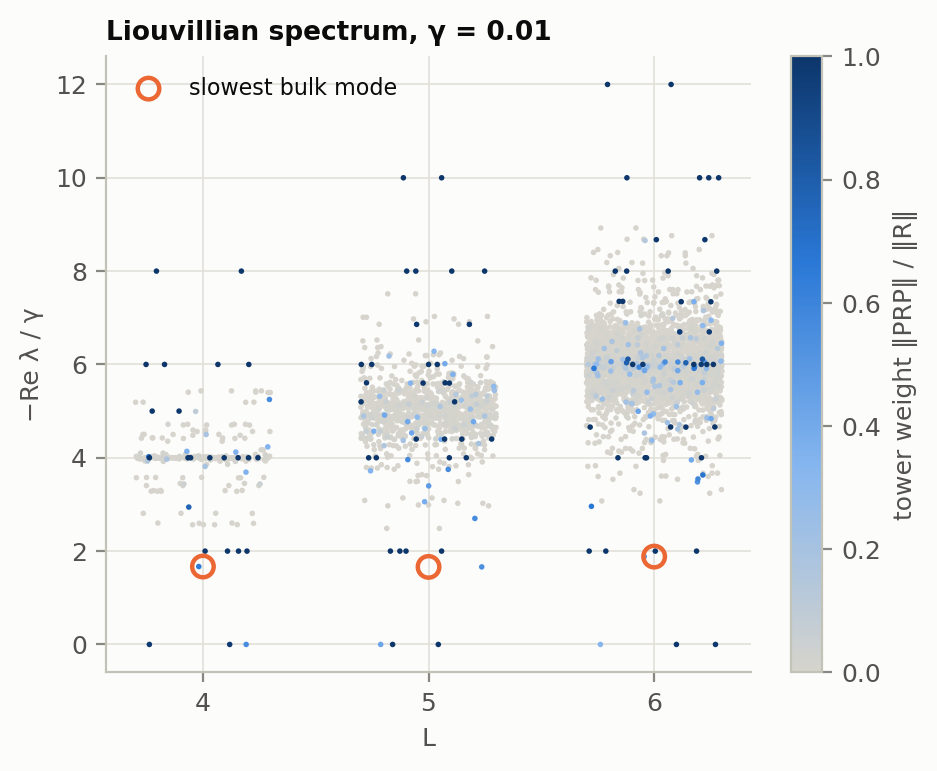
\includegraphics[width=0.62\textwidth]{spectrum.png}
\caption{$-\operatorname{Re}\lambda/\gamma$ of all Liouvillian modes, coloured by tower weight; circle: slowest bulk mode (\texttt{plot\_scripts/plot\_spectrum.py}).}
\label{fig:spectrum}
\end{figure}

%======================================================================
\section{Dependence on $\gamma$ at fixed $L = 6$}

Eleven values $\gamma = 0.002,\dots,6$, rates fitted on a window fixed in $\gamma t\in[0.05,0.6]$ (the window $[5,60]$ at $\gamma = 0.01$). A window fixed in $t$ samples different parts of the multi-exponential decay at different $\gamma$ and is not used here.

\begin{table}[h]
\centering
\small
\begin{tabular}{lccccccccccc}
\toprule
$\gamma$ & 0.002 & 0.005 & 0.01 & 0.02 & 0.05 & 0.1 & 0.2 & 0.5 & 1 & 3 & 6 \\
\midrule
P1 scar           & 4.80 & 4.78 & 4.69 & 4.61 & 4.59 & 5.67 & 3.75 & 2.47 & 2.14 & 2.02 & 2.00 \\
P2 energy         & 2.44 & 2.42 & 2.39 & 2.36 & 2.26 & 2.09 & 1.93 & 1.62 & 1.42 & 1.29 & 1.27 \\
P3 $\Delta\Gamma$ & 1.60 & 1.60 & 1.60 & 1.60 & 1.60 & 1.61 & 1.62 & 1.66 & 1.72 & 1.88 & 2.28 \\
\bottomrule
\end{tabular}
\caption{$\Gamma/\gamma$ at $L = 6$ (random $c$).}
\label{tab:gamma}
\end{table}

Three regimes for the scar (Fig.~\ref{fig:gamma}):
\begin{itemize}
\item \textbf{weak dephasing}, $\gamma\le0.05$: $\Gamma\propto\gamma^{0.984\pm0.002}$, i.e.\ linear, at $\approx4.7\gamma$;
\item \textbf{crossover} around $\gamma\approx0.1$, where $\gamma L\approx h$: a maximum $5.7\gamma$;
\item \textbf{strong dephasing}, $\gamma\gtrsim1$: $\Gamma\to2\gamma$; at $\gamma = 6$, $m_\perp(t) = e^{-2\gamma t}$ to $0.2\%$. The dephasing is much faster than $H_I$, so every spin dephases independently.
\end{itemize}
The non-scar rates are also linear in $\gamma$ for weak dephasing ($\gamma^{0.977}$ for P2, $\gamma^{1.001}$ for P3). At strong dephasing the energy probe slows down ($1.27\gamma$ at $\gamma = 6$), presumably because fast dephasing suppresses the coherent dynamics that moves weight out of the protected $S^z$-like content.

\begin{figure}[h]
\centering
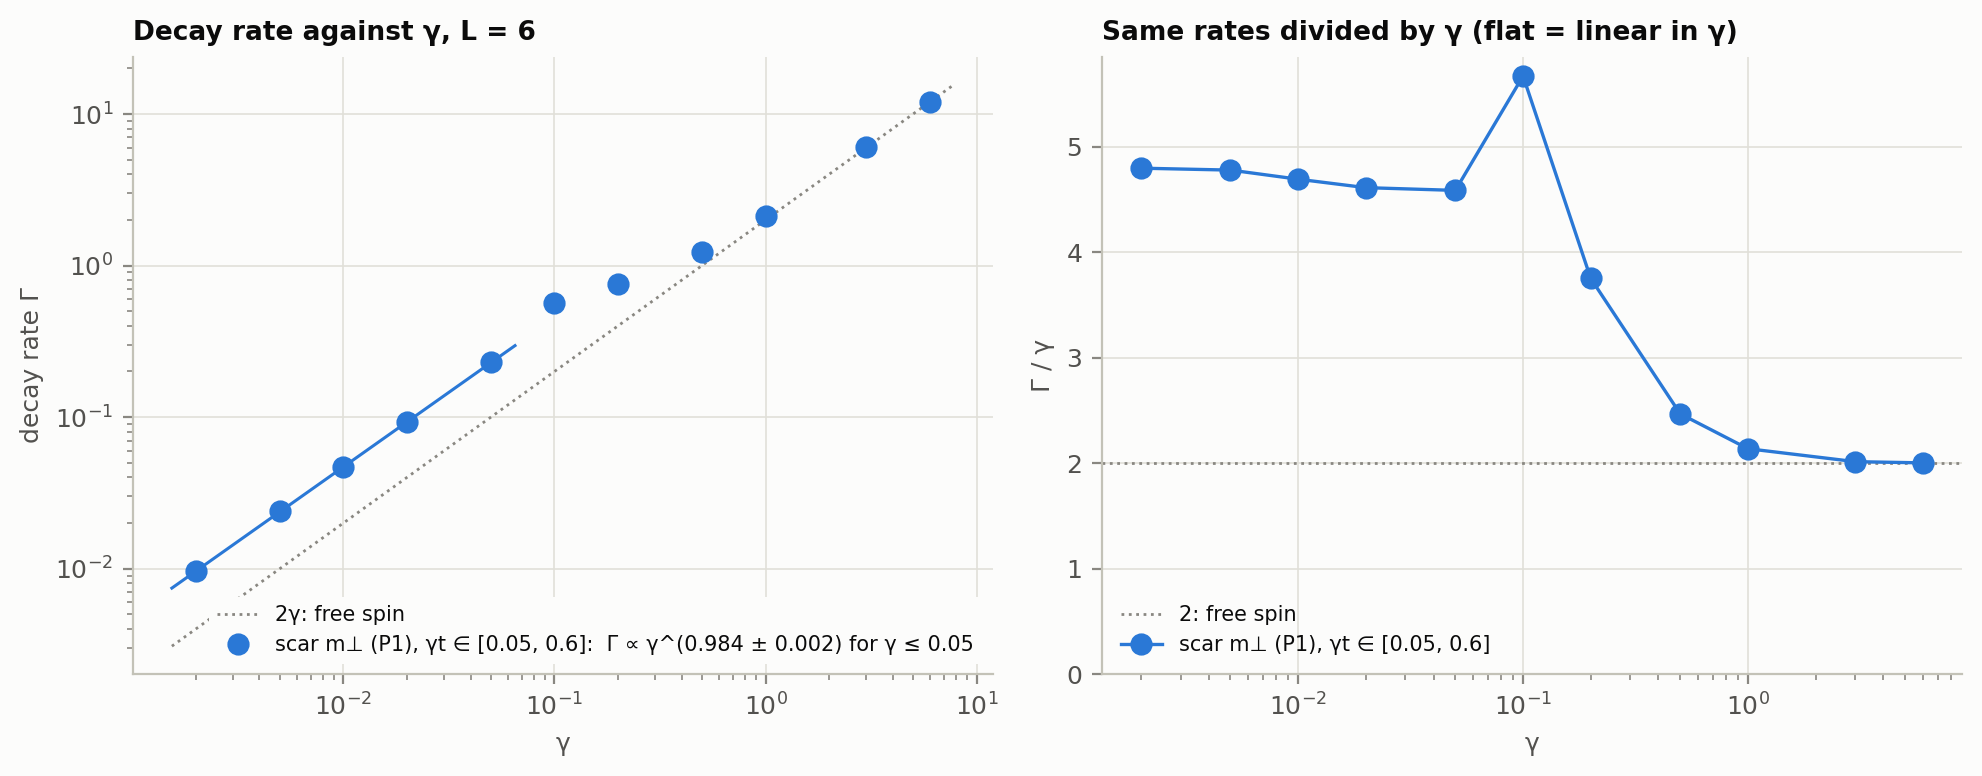
\includegraphics[width=\textwidth]{gamma_scan_scar.png}
\caption{Scar decay rate against $\gamma$ at $L = 6$; the power law is fitted for $\gamma\le0.05$ (\texttt{plot\_scripts/plot\_gamma\_scan.py}).}
\label{fig:gamma}
\end{figure}

\begin{figure}[h]
\centering
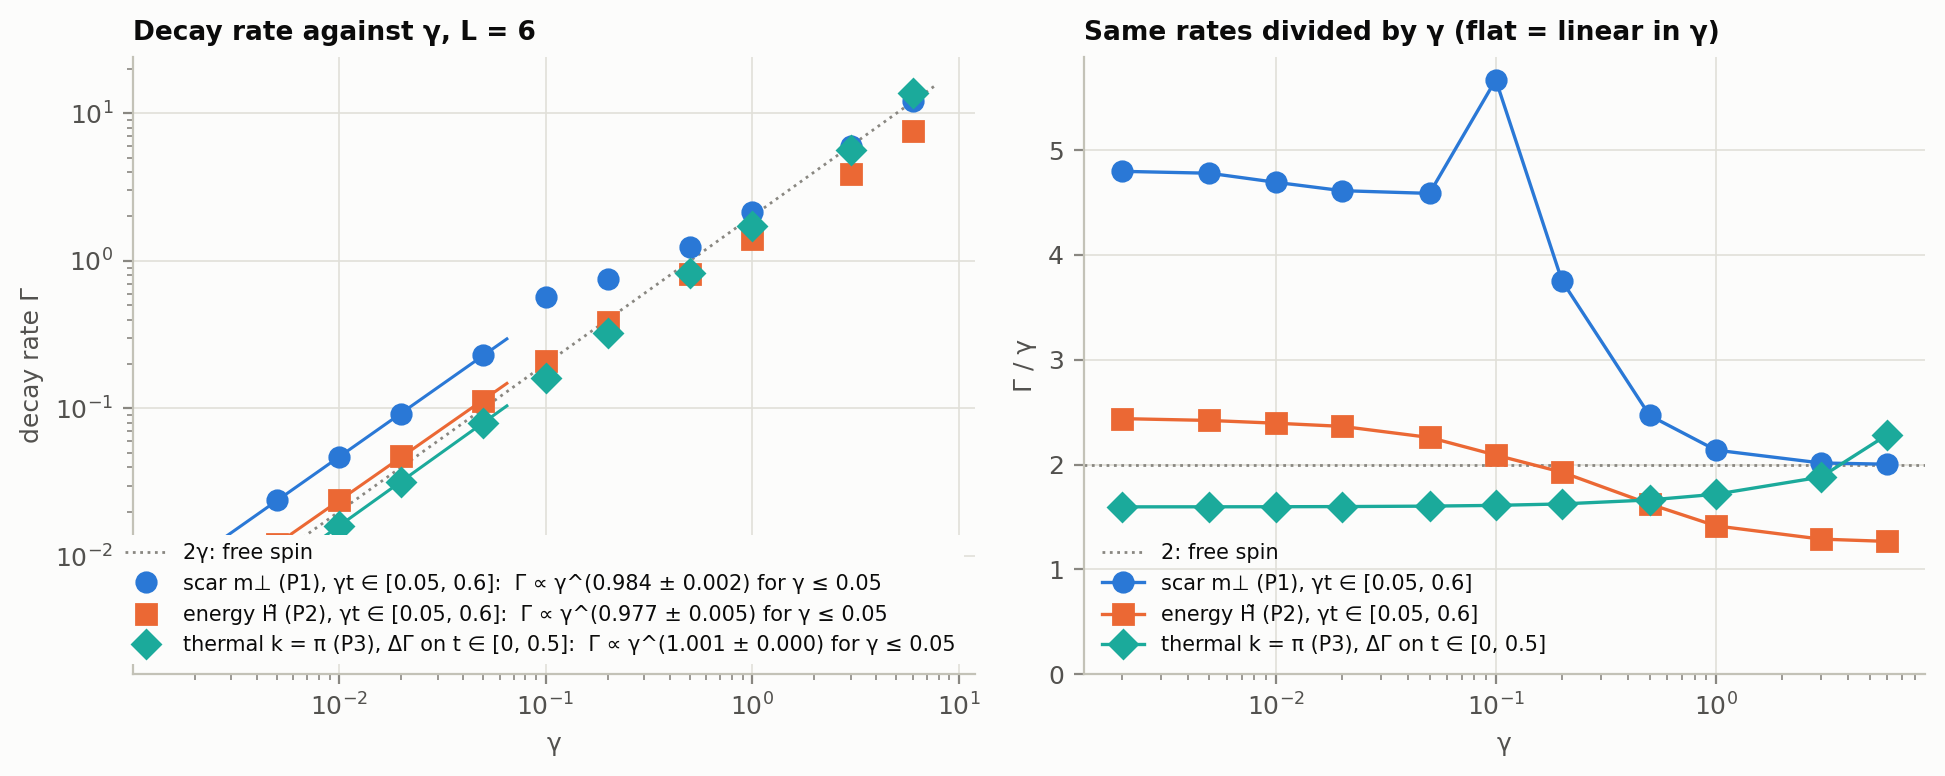
\includegraphics[width=\textwidth]{gamma_scan.png}
\caption{As Fig.~\ref{fig:gamma}, with the non-scar probes.}
\label{fig:gamma-all}
\end{figure}

%======================================================================
\section{Summary and open points}

\begin{itemize}
\item At $L\le8$ and weak dephasing, the scar oscillations decay at a rate growing roughly linearly with $L$ and linearly with $\gamma$; non-scar probes decay at $\approx2\gamma$, nearly independent of $L$. The $L$-growth is specific to the scar, consistent with the mid-tower coherences decaying at $\sim\gamma L$.
\item This growth is an early-time statement: the exact edge modes decay at $2\gamma$ for all $L$, and the late-time scar decay drifts towards them. Whether the local revival envelope has an $L$-independent rate in the $L\to\infty$-first limit is not decided by $L\le8$.
\item The steady state is three-fold degenerate (dark fully polarized states); the project notes assumed uniqueness.
\item Open: more disorder realizations; larger $L$ with trajectories; a fit-free observable (e.g.\ the weights of the exact eigenmodes in $m_\perp$) instead of window-dependent rates; the order of limits $\gamma\to0$, $L\to\infty$.
\end{itemize}

\end{document}
